\documentclass[10pt]{article}
\usepackage[]{graphicx}\usepackage[]{color}
\makeatletter
\def\maxwidth{ %
  \ifdim\Gin@nat@width>\linewidth
    \linewidth
  \else
    \Gin@nat@width
  \fi
}
\makeatother

\usepackage{Sweavel}
\usepackage{hyperref}
\usepackage{url}
\usepackage[a4paper]{geometry}
\usepackage{a4wide}
\usepackage{float}
\usepackage[english]{babel}
\usepackage[utf8]{inputenc}
\usepackage{csquotes}
\usepackage{amsmath}
\usepackage{amssymb}
\usepackage{xspace}
\usepackage[numbers]{natbib}
\bibliographystyle{unsrtnat}
\usepackage{subcaption}
\usepackage[font={small}]{caption}
\usepackage{booktabs}
\usepackage{listings}
\usepackage{cleveref}
\usepackage{lipsum}
\newcommand{\approxtext}[1]{\ensuremath{\stackrel{\text{#1}}{=}}}
\newcommand{\matr}[1]{\mathbf{#1}}
\newcommand{\partt}[2]{\ensuremath{\dfrac{\partial {#1}}{\partial {#2}}}}
\renewcommand{\d}[1]{\ensuremath{\operatorname{d}\!{#1}}} % non-italized differentials
\newcommand{\h}[0]{\ensuremath{\hbar}} % hbar
\def\changemargin#1#2{\list{}{\rightmargin#2\leftmargin#1}\item[]}
\let\endchangemargin=\endlist 
\usepackage{amsthm}
\theoremstyle{plain}
\renewcommand{\theequation}{\thesection.\arabic{equation}}
\def\changemargin#1#2{\list{}{\rightmargin#2\leftmargin#1}\item[]}
\let\endchangemargin=\endlist    
\usepackage{xcolor}
\definecolor{Red}{rgb}{0.7,0,0}
\definecolor{Blue}{rgb}{0,0,0.8}
\usepackage{verbatim}
\def\changemargin#1#2{\list{}{\rightmargin#2\leftmargin#1}\item[]}
\let\endchangemargin=\endlist
\addtolength{\oddsidemargin}{-.35in}
\addtolength{\evensidemargin}{-.35in}
\addtolength{\textwidth}{.7in}
\usepackage{multicol}

% Stephen's stuff
\newcommand{\R}{\texttt{R}}
\newcommand{\Rfunction}[1]{{\texttt{#1}}}
\newcommand{\Robject}[1]{{\texttt{#1}}}
\newcommand{\Rpackage}[1]{{\mbox{\normalfont\textsf{#1}}}}
\usepackage{xcolor}
\definecolor{Red}{rgb}{0.7,0,0}
\definecolor{Blue}{rgb}{0,0,0.8}
\hypersetup{%
pdfusetitle,
bookmarks = {true},
bookmarksnumbered = {true},
bookmarksopen = {true},
bookmarksopenlevel = 2,
unicode = {true},
breaklinks = {false},
hyperindex = {true},
colorlinks = {true},
linktocpage = {true},
plainpages = {false},
linkcolor = {Blue},
citecolor = {Blue},
urlcolor = {Red},
pdfstartview = {Fit},
pdfpagemode = {UseOutlines},
pdfview = {XYZ null null null}
}
%% Listings
\lstset{ 
language=R,                     % the language of the code
basicstyle=\footnotesize,       % the size of the fonts that are used for the code
numbers=left,                   % where to put the line-numbers
numberstyle=\tiny\color{gray},  % the style that is used for the line-numbers
stepnumber=1,                   % the step between two line-numbers. If it's 1, each line will be numbered
numbersep=5pt,                  % how far the line-numbers are from the code
backgroundcolor=\color{white},  % choose the background color. You must add \usepackage{color}
showspaces=false,               % show spaces adding particular underscores
showstringspaces=false,         % underline spaces within strings
showtabs=false,                 % show tabs within strings adding particular underscores
rulecolor=\color{black},        % if not set, the frame-color may be changed on line-breaks within not-black text (e.g. commens (green here))
tabsize=2,                      % sets default tabsize to 2 spaces
captionpos=b,                   % sets the caption-position to bottom
breaklines=true,                % sets automatic line breaking
breakatwhitespace=false,        % sets if automatic breaks should only happen at whitespace
title=\lstname,                 % show the filename of files included with \lstinputlisting;
% also try caption instead of title
keywordstyle=\color{Blue},      % keyword style
commentstyle=\color{orange},    % comment style
stringstyle=\color{Red},        % string literal style
escapeinside={\%*}{*)},         % if you want to add a comment within your code
morekeywords={*,...}            % if you want to add more keywords to the set
} 


%%% Document specific
\newcommand{\course}{Biological Imaging and Analysis}
\newcommand{\ass}{1}
\newcommand{\term}{Easter term 2017}

%%% Title page
\title{
  \bf \course: Assignment \ass \\[1em]
  \small{University of Cambridge}
}
\newcommand{\specialcell}[2][c]{%
  \begin{tabular}[#1]{@{}c@{}}#2\end{tabular}}

\author{Henrik Åhl}
\date{\today}
\renewcommand{\textfraction}{0.05}
\renewcommand{\topfraction}{0.8}
\renewcommand{\bottomfraction}{0.8}
\renewcommand{\floatpagefraction}{0.75}

%%% Actual document
\begin{document}
\date{\today}
\maketitle
\setcounter{page}{1}
\maketitle

\begin{multicols*}{2}
\section*{Preface}
This is an assignment report in connection to the \textit{\course}
module in the Computational Biology course at the University of Cambridge,
\term. All related code is as of \date{\today} available through a
Github repository by contacting \href{mailto:hpa22@cam.ac.uk}{hpa22@cam.ac.uk}.

\subsection*{1: Calculating the volume of a mouse embryo}
The applied algorithm consists of applying in succession a range of tools in order to improve upon the analysis. The first things we do is to prune off the last 10 slices of our stack, since these appear to only contain background noise and not any direct cell matter \textit{per se}. It also makes to stack slightly less asymmetric, as the first slice begins in middle of a layer of cells. With this more representative stack, we for all the subsequent applied tools use the middle slice, i.e.\ slice 50, as the baseline. As this is approximately in the middle of the tissue and ought to be fairly representative. 

We thereafter despeckle the image, which applies a median filter supposed over a $3\times3$ pixel surface, with the intention of removing salt-and-pepper noise, i.e.\ single, individual bright or dark spots. The median filter itself simply takes out the median of the nine cells and sets all of the cells to this value. In order to smoothen the result, we thereafter apply a simple gaussian filter with $\sigma = 2$, which produces a gaussian kernel, or convolution matrix, in accordance to the equation $$g(x, y) = \dfrac{1}{\sigma \sqrt{2\pi}}\exp^{-\dfrac{x^2 + y^2}{2\sigma^2}}$$, where $\sigma$ is the rate of decay for the kernel. Every pixel is then replaced with the sum of the kernel elements multiplied correspondingly with the pixel's vicinity, with the kernel centered on the pixel~\cite{imagej_methods}. 

$x$ and $y$ being the cartesian distances to the origion. $\sigma$ the standard deviation of the change. Since we thereafter want to find the maxima of our cells in order to identify them using the \texttt{3D Find Maxima} function, we apply a maximum filter, which effectively is analogous to the median filter. In some of our cases we want to reduce the amount of noise in the image further, and therefore apply a \texttt{Remove Outliers} filter of radius 10 and threshold 0, which replaces pixels with the median of surrounding pixels if it deviates by more than the defined threshold. In other words, we filter out large chunks where cells have merged and become indistinguishable, as well as aberrant spots outside of the embryo~\cite{imagej_methods}. 

The resulting image is then thresholded at slice 50 with either the Li or the Otsu method. Li's method minimises the cross-entropy between the threshold and the original image, whereas Otsu's method minimises the weighted variance between the thresholded and the original. In the case of Li's method, the cross-entropy takes the form of
$$ \eta(t) = -m_{1fore}(t)\log\dfrac{m_{1fore}(t)}{m_{0fore}(t)} -m_{1back}(t)\log\dfrac{m_{1back}(t)}{m_{0back}(t)},$$
where the m's are the zeroth and first order moments of the foreground and background parts of the image respectively~\cite{li}. 

Otsu's method can be described as minimising the function $$\sigma^2 = W_{back}\sigma_{back}^2 + W_{fore}\sigma_{fore}^2,$$ 
where the weights correspond to the normalised frequencies of the foreground and background intensities, and the $\sigma$s simply the standard deviations~\cite{otsu}. 


In \cref{fig:2_maxima_1,fig:2_maxima_2} we see the inferred maxima from our approaches, with the parameter settings described in \cref{tab:params}. The idea here is of course that cell maxima should correspond to the cells themselves, although as we can see, the inferred number of cells vary wildly between the analyses. Comparing this to \cref{fig:2_threshold_1,fig:2_threshold_2}, which are the images on which the \texttt{Find Maxima} functio has been applied, we see that they do not differ significantly from each other visually. This naturally raises the importance of post-simulation analysis, with double-checking where the identified maxima are, and whether they correspond to actual cells. We can note some interesting features of our applied tools, however. For example, applying the \texttt{Remove Outliers filter} has indeed helped with misclassifying spots outside of the embryo as cells, as the differences between figures $A-D$ and $E-G$ shows. It is also not a significant factor in bringing down the number of inferred cells, which indeed is governed primarily by the assumed maxima radius, which we have exemplified by setting a lower value in one dimension. A major part of the analysis therefore comes down to accurately estimating an average cell size. Since we do have some visual artifacts making it hard to measure cell size in the $z$ direction, the perhaps most accurate approach would be to assume spherical cells. When we do so, we arrive at ca 10000 cells, which appears visually reasonable.

\begin{table*}[t]
\centering
\caption{Table description of the different simulations and their corresponding input parameters and results, using a blob size of 17 $\mu m$.}
\label{tab:params}
\begin{tabular}{@{} *8c @{}}\toprule
\emph{Figure} & \emph{RO radius} & \emph{Maxima radius} & \emph{Gaussian $\sigma$}& \emph{xy} & \emph{$z$ } & \emph{No.\ maxima, Li} & \emph{No.\ maxima, Otsu}\\\midrule
  A & N/A & 6 & 2   & 6 & 1.5 & 28442 & 19900\\
  B & N/A & 6 & N/A & 6 & 1.5 & 12754 & 10627\\
  C & N/A & 6 & 2   & 6 & 6.0 &  6917 &  5238\\
  D & N/A & 6 & N/A & 6 & 6.0 &  4465 &  4022\\
  E & 10  & 6 & 2   & 6 & 1.5 & 24758 & 18254\\
  F & 10  & 6 & N/A & 6 & 1.5 & 11393 &  9678\\
  G & 10  & 6 & 2   & 6 & 6.0 &  5247 &  4320\\
  H & 10  & 6 & N/A & 6 & 6.0 &  3545 &  3259\\\bottomrule
\hline
\end{tabular}
\end{table*}

\end{multicols}
\newpage
\begin{Schunk}
\begin{figure}[H]

{\centering \includegraphics[width=\maxwidth]{figure/twocolumn-2_maxima_1-1} 

}

\caption[Identified maxima as produced by the Li thresholding method]{Identified maxima as produced by the Li thresholding method.}\label{fig:2_maxima_1}
\end{figure}
\end{Schunk}
\phantom{p}
\vspace*{\fill}
\begin{Schunk}
\begin{figure}[H]

{\centering \includegraphics[width=\maxwidth]{figure/twocolumn-2_maxima_2-1} 

}

\caption[Identified maxima as produced by the Otsu thresholding method]{Identified maxima as produced by the Otsu thresholding method.}\label{fig:2_maxima_2}
\end{figure}
\end{Schunk}
\vfill
\newpage
\phantom{p}
\vspace*{\fill}
\begin{Schunk}
\begin{figure}[H]

{\centering 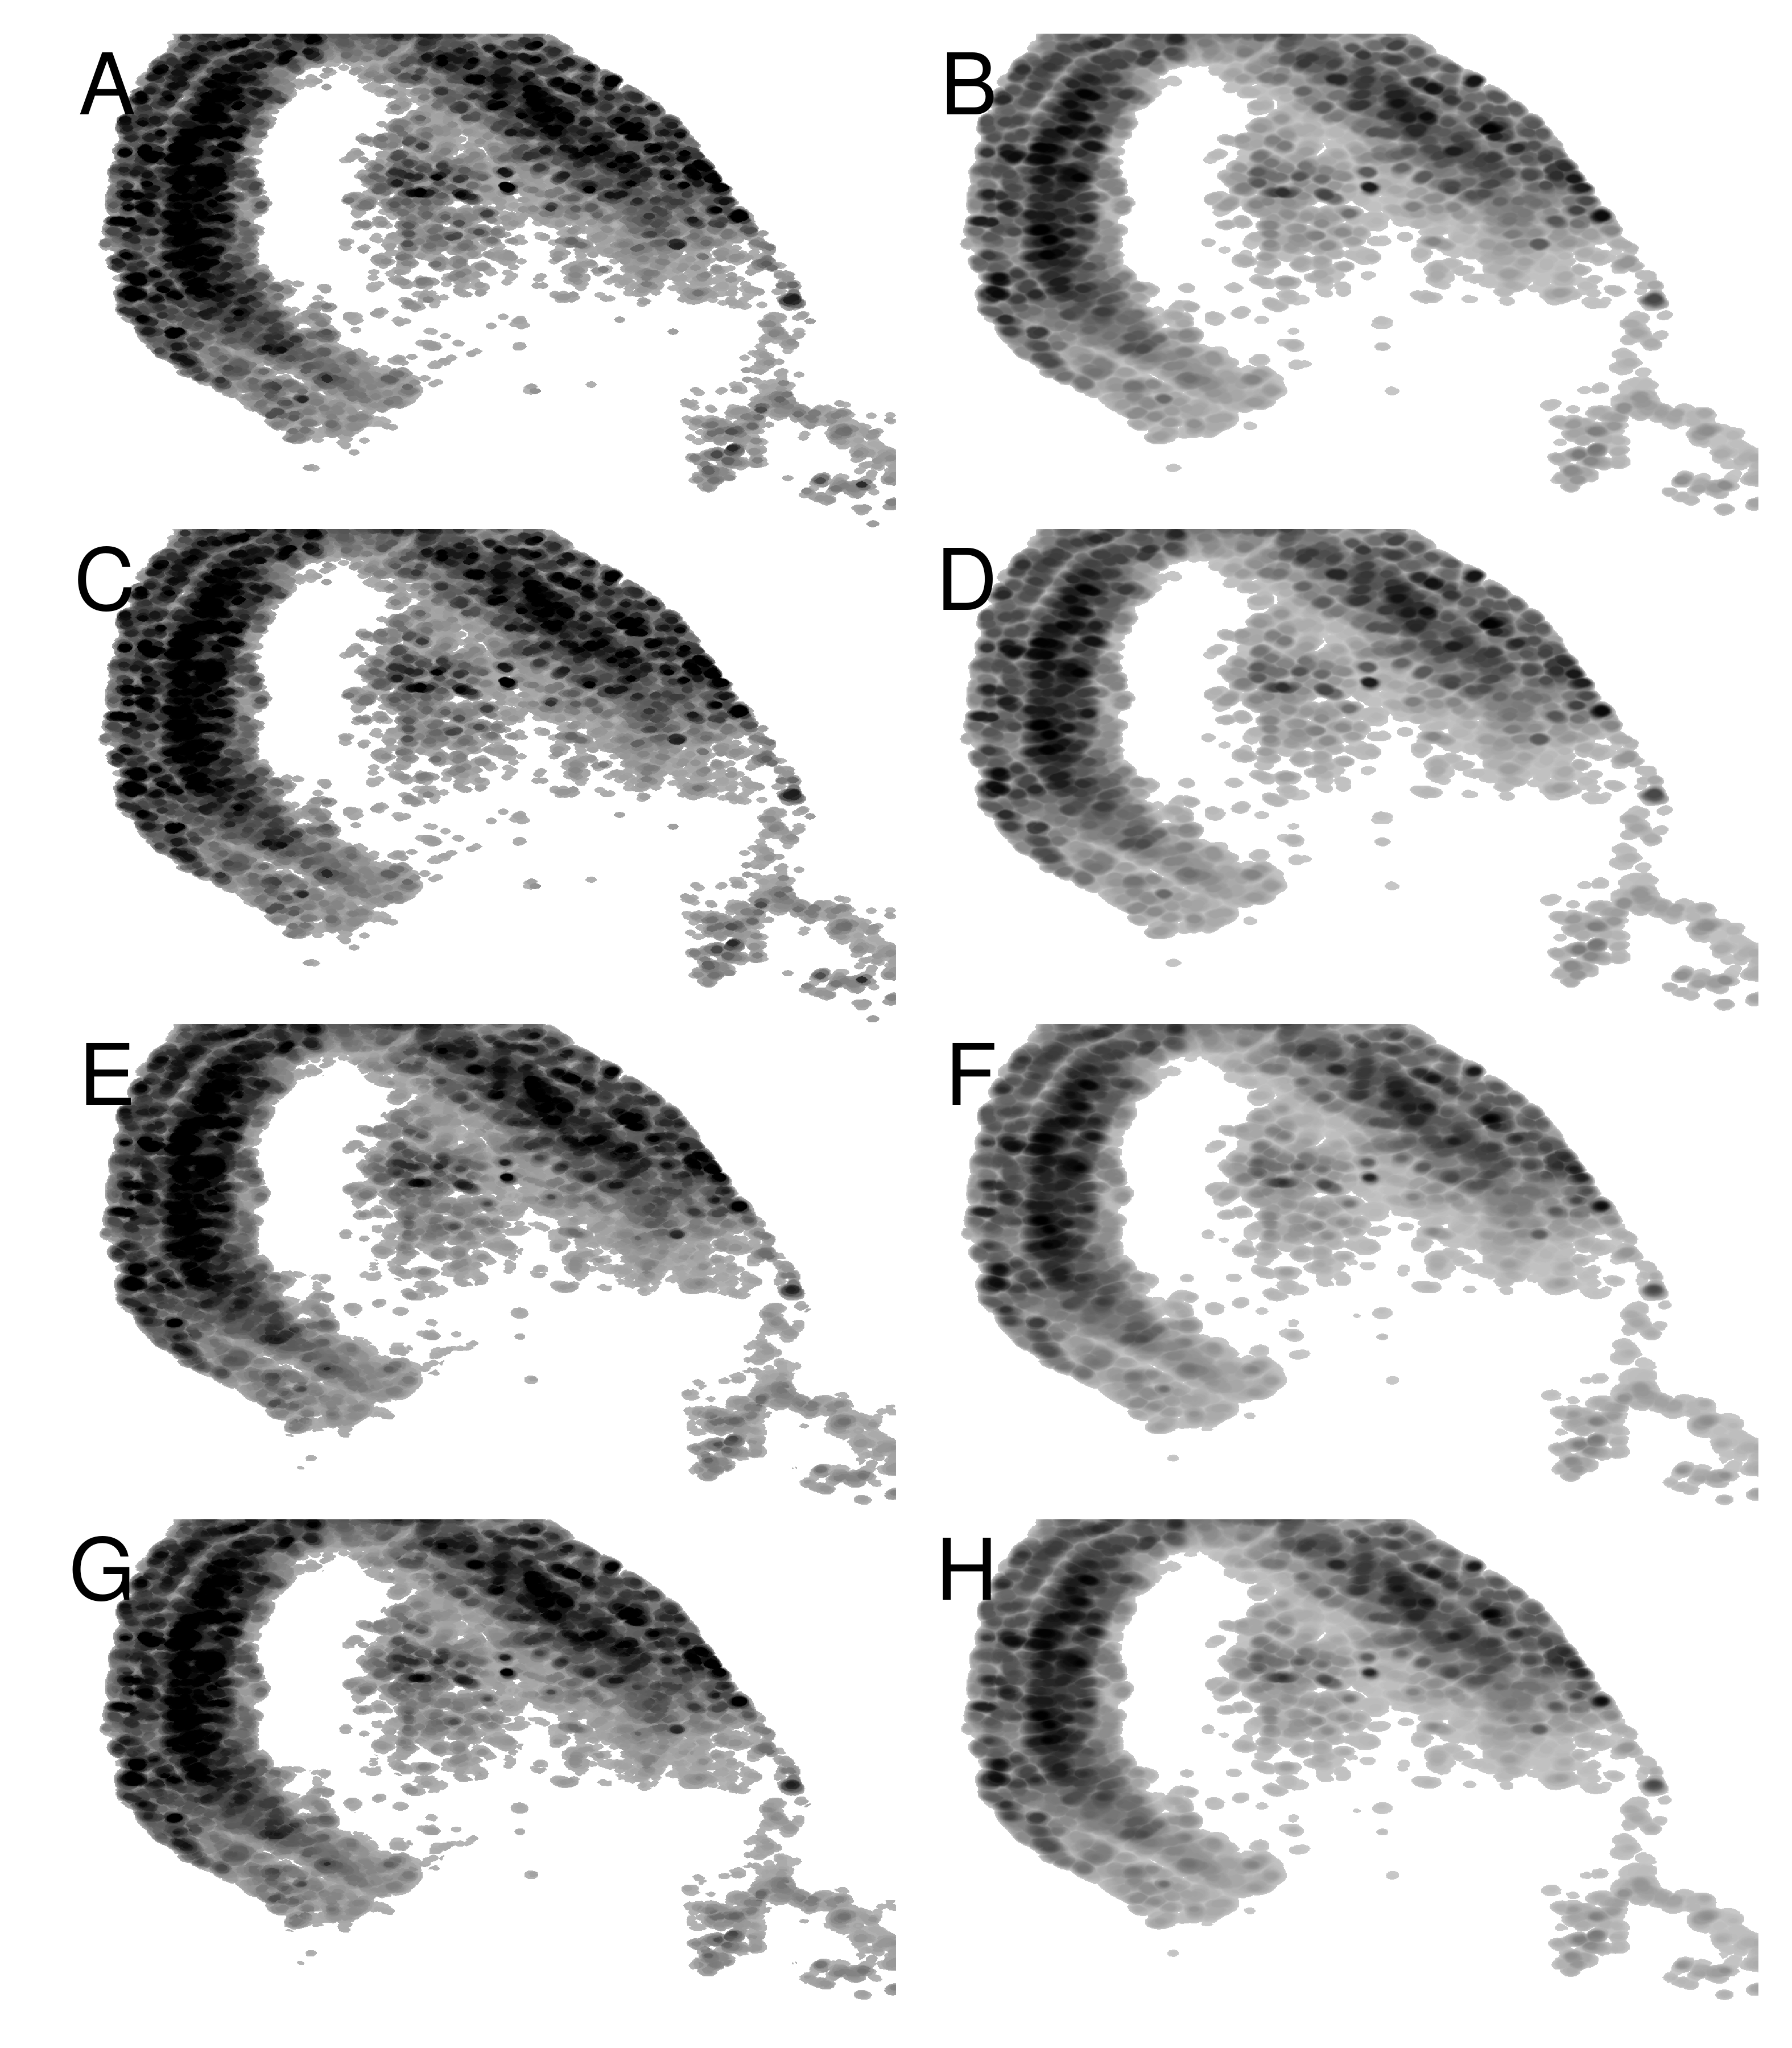
\includegraphics[width=\maxwidth]{figure/twocolumn-2_threshold_1-1} 

}

\caption[Li threshold]{Li threshold. Thresholded and multiplied filtered image. Darker dots represent higher intensities.}\label{fig:2_threshold_1}
\end{figure}
\end{Schunk}
\vfill
\newpage
\phantom{p}
\vspace*{\fill}
\begin{Schunk}
\begin{figure}[H]

{\centering 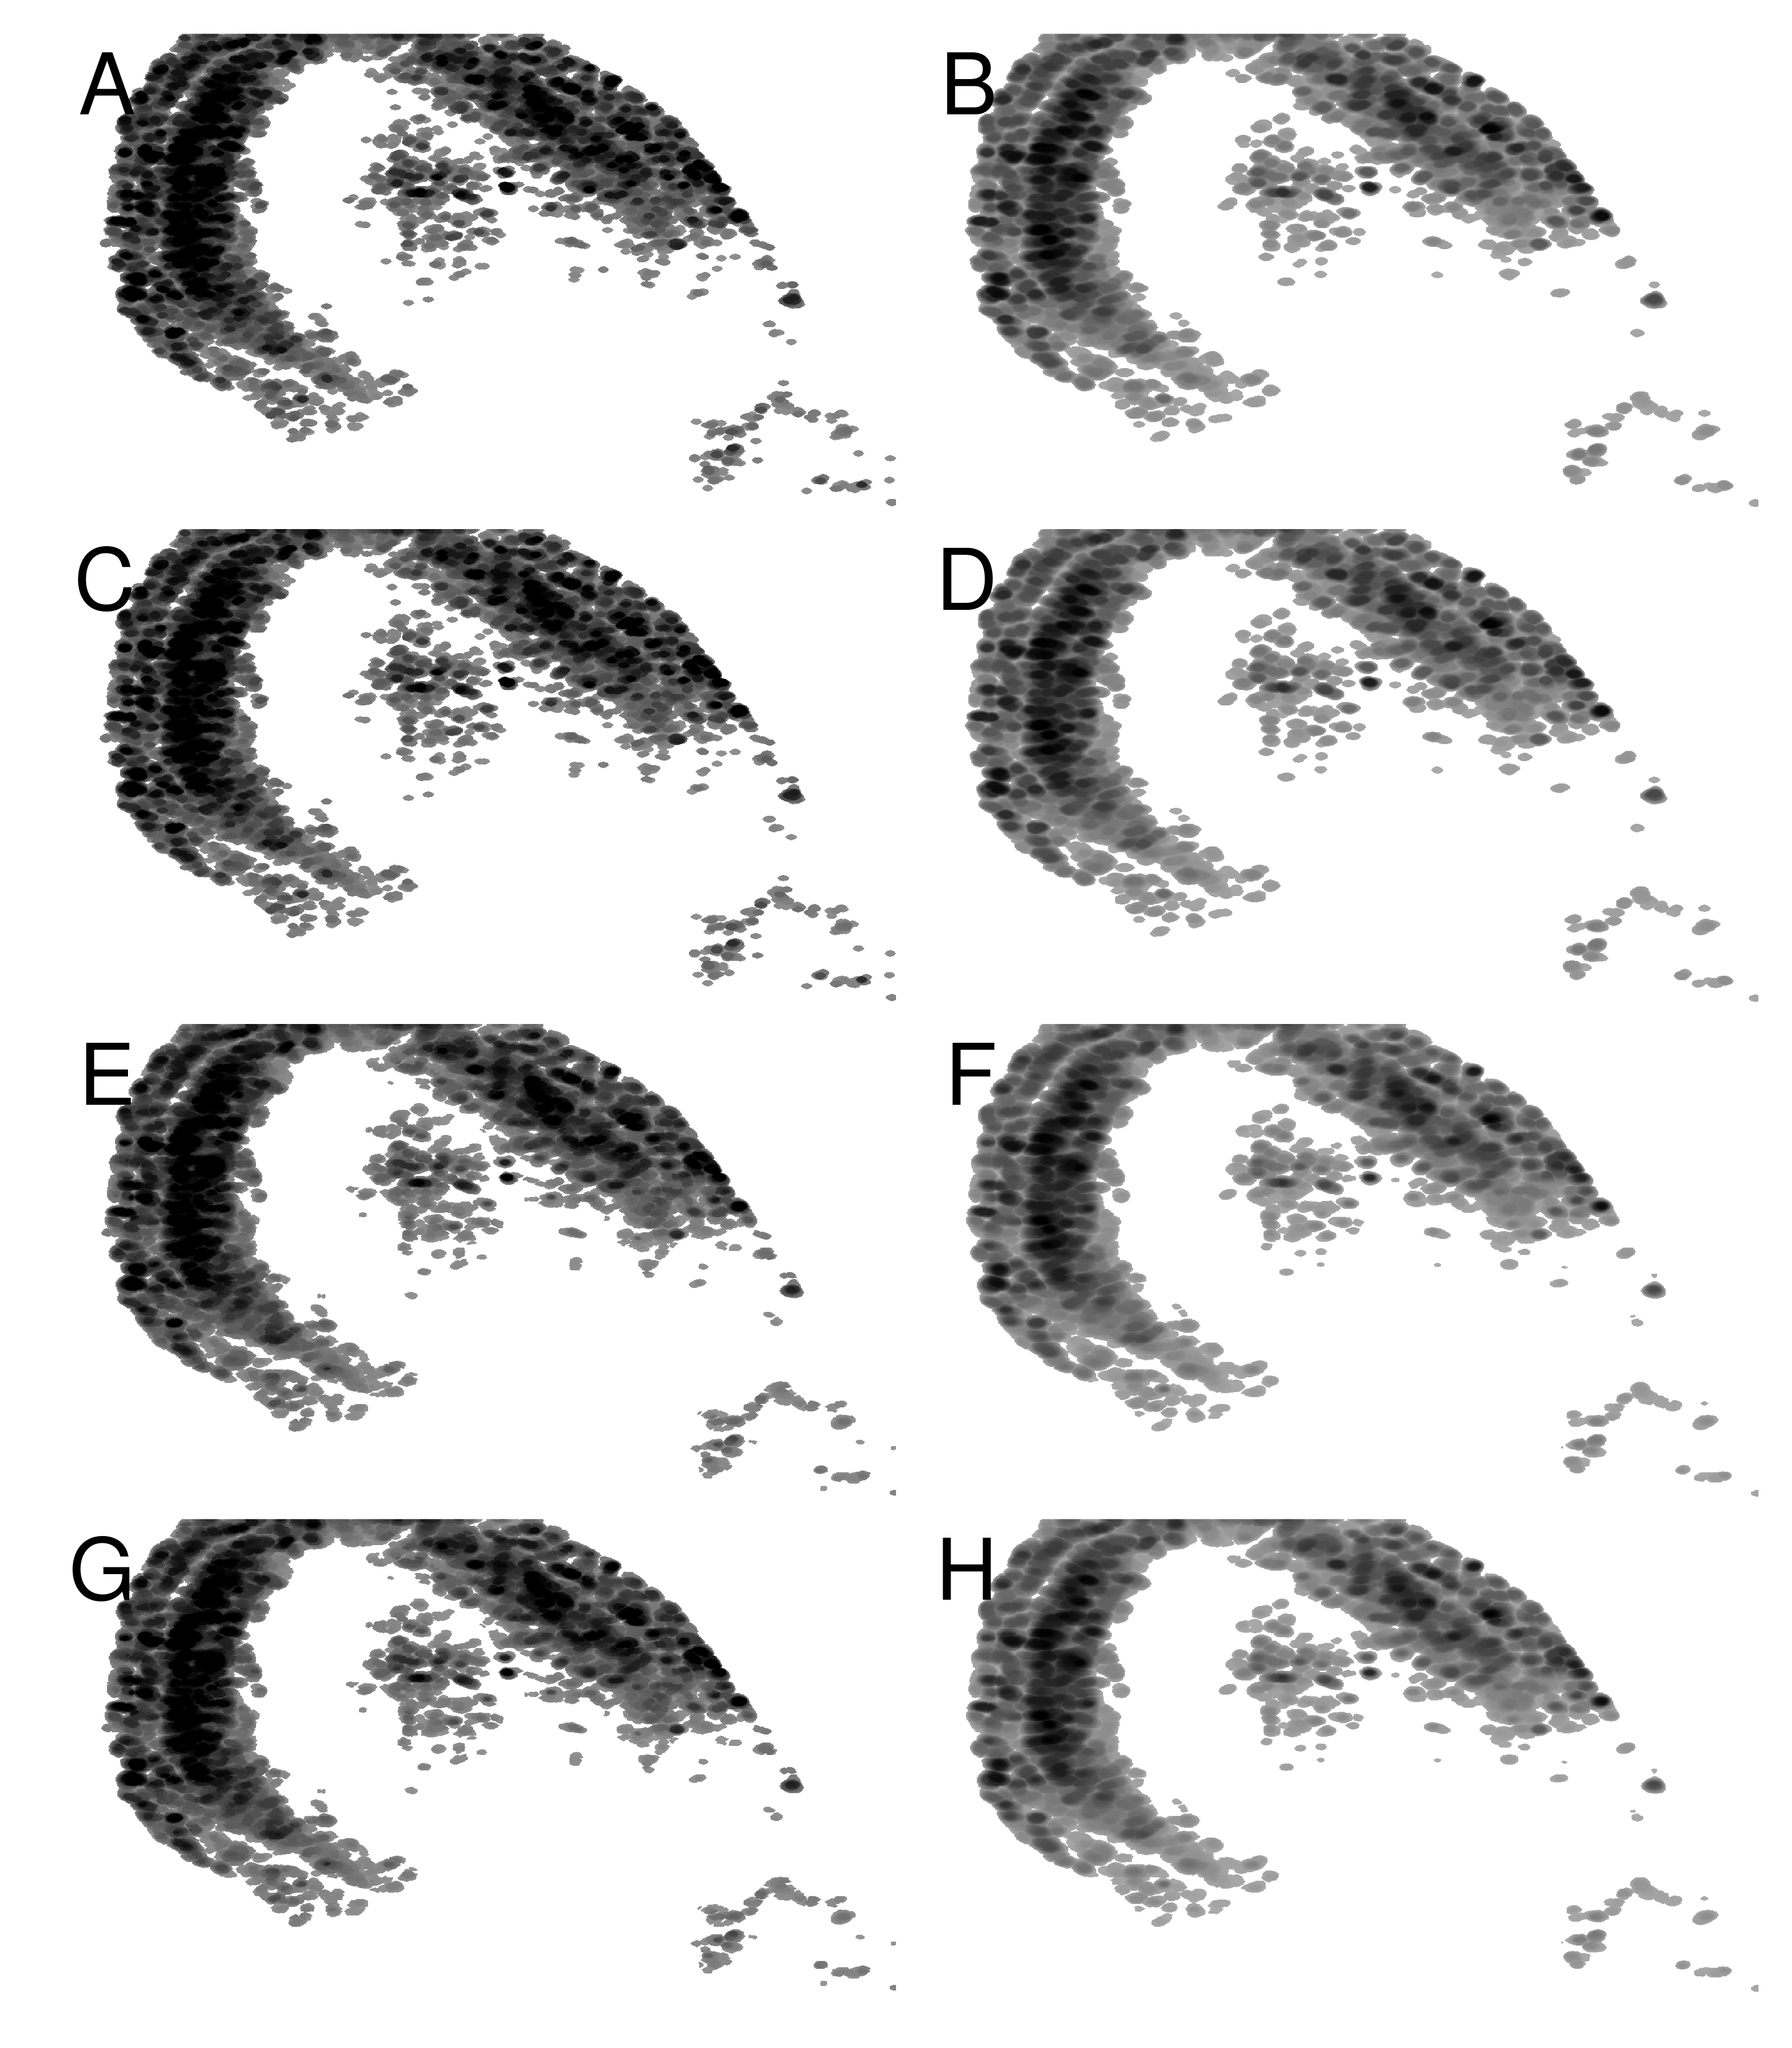
\includegraphics[width=\maxwidth]{figure/twocolumn-2_threshold_2-1} 

}

\caption[Otsu threshold]{Otsu threshold. Thresholded and multiplied filtered image. Darker dots represent higher intensities.}\label{fig:2_threshold_2}
\end{figure}
\end{Schunk}
\vfill
\newpage

\begin{multicols}{2}
When we disregard counting the cells directly through the measured maxima and instead try to infer the number of cells through calculation of the volume, we get the results seen in \cref{fig:2_no_cells}. Here we used the same thresholded images as previously, but instead of modifying our processed image with it, we calculate the volume occupied by the thresholded chunk. As we clearly can see, $Li's$ method is less generous with which values are included when performing the threshold, as the volume is consistently smaller than for Otsus's method. The choice of method is therefore clearly very important when doing such an approximation, and we can correspondingly also expect large variances in our estimate of the number of cells from this. Being very rough, we can get the number of cells from the volume by estimating the volume of a single cell, and simply dividing the volume calculated from the thresholded image by this. Doing so is precisely what gives us the cell number estimate in \cref{fig:2_no_cells}, where we have assumed a cell to be sperical with a radius of $6$ pixels, which was concluded by manually measuring a set of cells. While this approach is naturally very inexact, it gives us an idea of the order of magnitude of the total number, which appears to be on the order of 10000. 


\begin{Schunk}
\begin{figure}[H]

{\centering 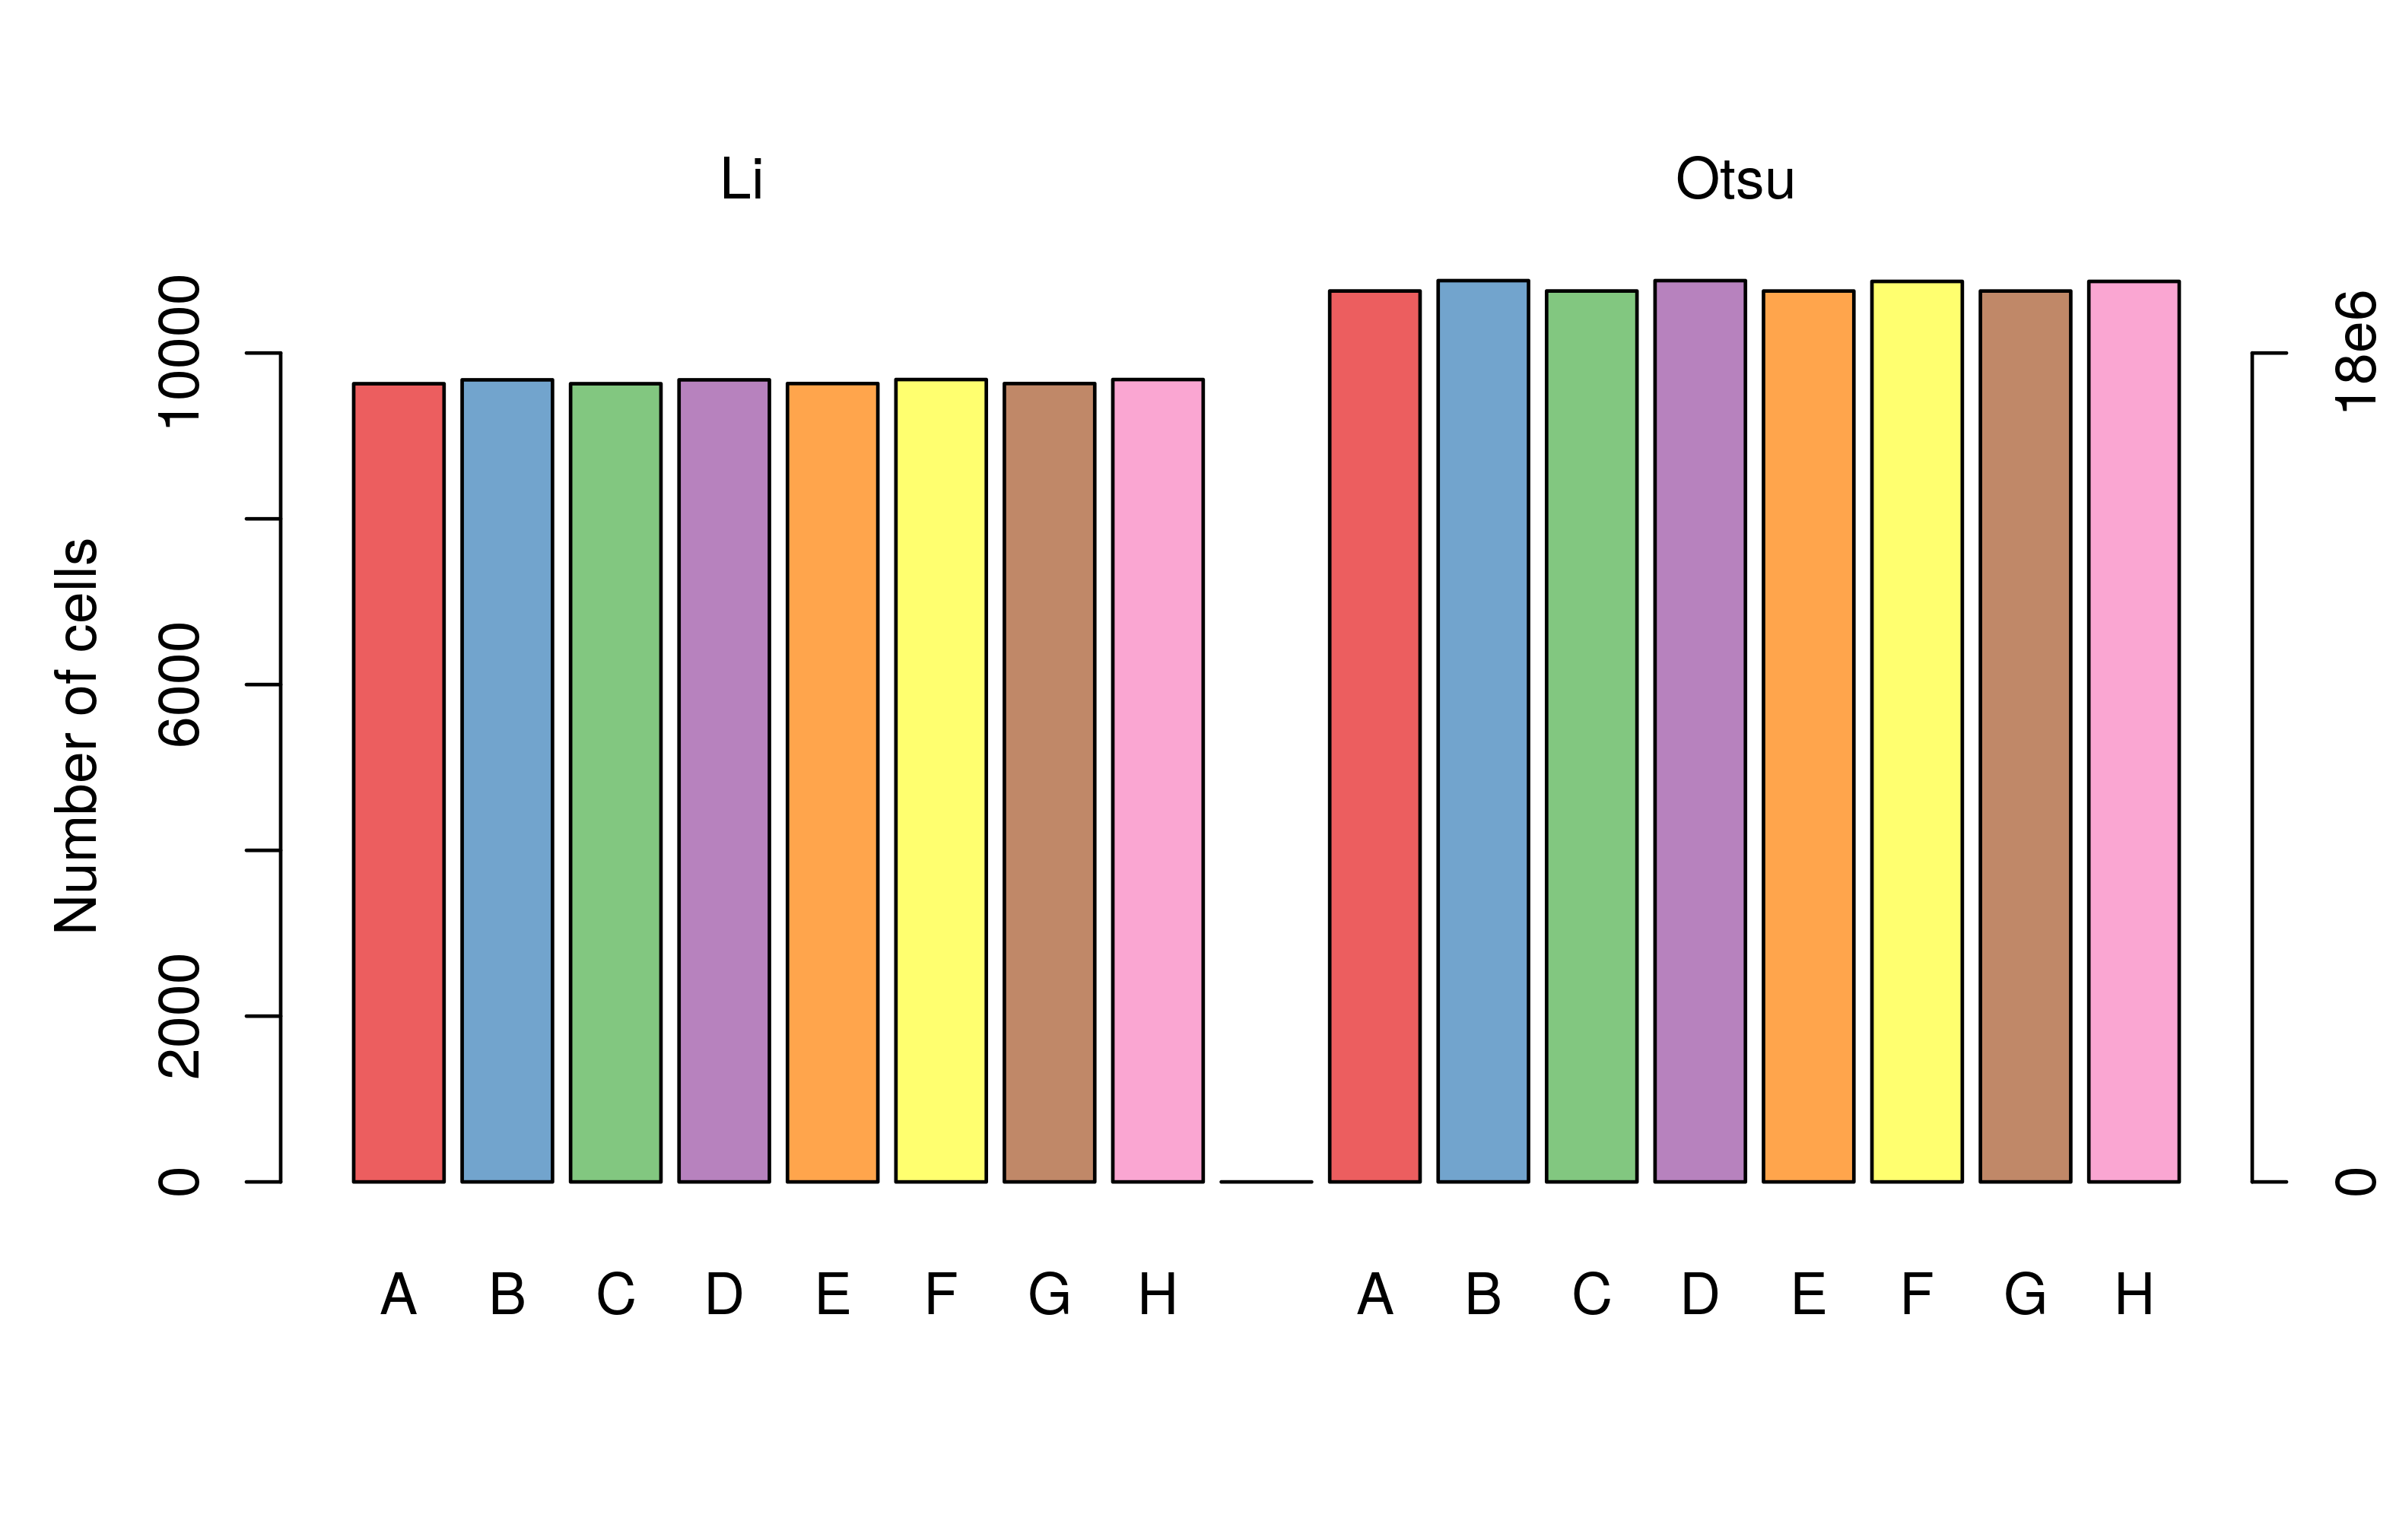
\includegraphics[width=\maxwidth]{figure/twocolumn-2_no_cells-1} 

}

\caption[Otsu threshold]{Otsu threshold. Thresholded and multiplied filtered image. Darker dots represent higher intensities.}\label{fig:2_no_cells}
\end{figure}
\end{Schunk}

In both of our attempts, we must however note that we are working with DAPI staining, which binds to the nuclear envelope, and not to the cell wall itself. We are therefore bound to underestimate the volume by default. 

% We only see the nuclear envelope -- not the cells. So what is the area of the embryo? We don't really know. 


\subsection*{2: Tracking cells using TrackMate}
In our second assignment we track a set of Histone 2B expressing cells using epifluorescence microscopy time-series data. Before initialising the tracking, we modify our images brightness and contrast significantly, in order to identify cells not visible at first glance. To safety check, we perform manual counting on the inital frame, where our method is indeed able to locate all 48 cells there from the beginning. The figure corresponding to this is seen in \cref{fig:contrasts}. Note in particular the dark spots appearing in several places on the picture. Most of these, if not all, correspond to imaging artifacts, such as stains on the microscope lens or the likes. For several attempts to track our cells, these spots are wrongly identified as cells themselves, and we therefore choose to remove these with a twice applied \texttt{Remove Outliers} filtering. Similarly, due to the graininess of the image, we also do this once for white spots with a radius of 1.
% HOW DOES THIS WORK? 
 
\begin{figure}[H]
  \centering
  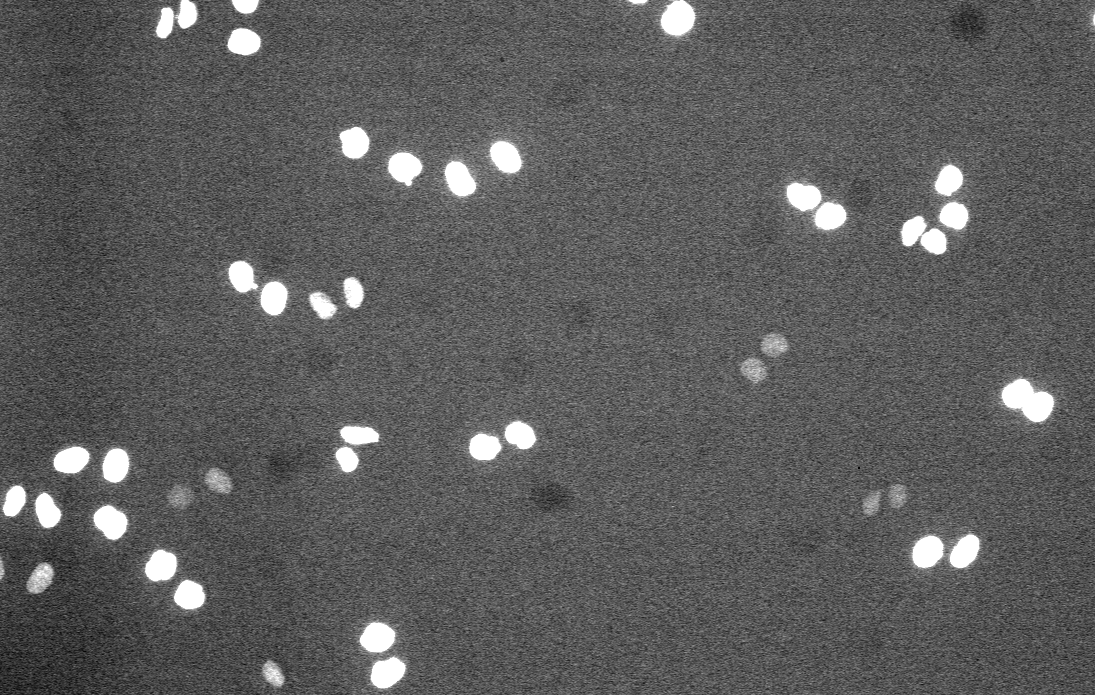
\includegraphics[width=.5\textwidth]{../figures/contrast.png}
  \caption{Image showing the initial frame after modifying contrasts. Note in particular the two dim cells in the bottom right corner, as these prove to be particularly hard to identify throughout. Also note the black stains, which correspond to imaging artifacts.}
  \label{fig:contrasts}
\end{figure}

Using TrackMate, we perform the built-in automated median filtering without thresholding, and set the estimated blob diameter to 15~$\mu$m. This is an under-estimate, but done in order to not lose track of cells undergoing mitosis, as well as cells who give of low fluorescence. Since we work with nuclear staining, the identified objects occasionally vary significantly in size between frames. In particular during mitosis we can see how the chromosomes align, as this causes the cells to occur only as a thin, elongated stripes. 

After identification of potential cells to track through a Laplacian of Gaussians (LoG) segmentation, which transforms all the pixels using the LoG equation $$LoG(x,y) = - \dfrac{1}{4\pi\sigma}\left(1 - \dfrac{x^2 + y^2}{2\sigma^2}\right)\exp^{-\dfrac{x^2 + y^2}{2\sigma^2}},$$ effectively enhancing the outline of the cell. From this we filter based on inferred quality, which is a predefined metric used by the $LoG$ kernel precisely for blob detection.  

The cells are tracked using the \textit{LAP tracker}, which is supposed to be ideal for particles undergoing brownian motion, as we assume ours are. Since our images appear to allow for some jumping of our cells between frames, it occasionally happens that a cell division is mischaracterised as a new cell occuring from elsewhere. However, this appears to happen mostly in fringe cases, such as for the top-central, massive blob, which is a hard enough classification as is. We nevertheless choose to increase the frame-frame linkage to a distance of 20~$\mu$m, as well as set the splitting distance to 30 $\mu$m. Visually, this appears to give us better results. We also increase the maximum frame gap to 4, as cells sometimes merge in such a way that the segmenter are unable to recognise them individually. Due to this, it sometimes happens that cells are somethimes inferred to be part of an incorrect track; however, this seems like an unavoidable issue that cannot be resolved without fine-tuning cell trajectories manually. In addition, it does not affect our results, as we filter out tracks with disappearing members. 

\begin{Schunk}
\begin{figure}[H]

{\centering 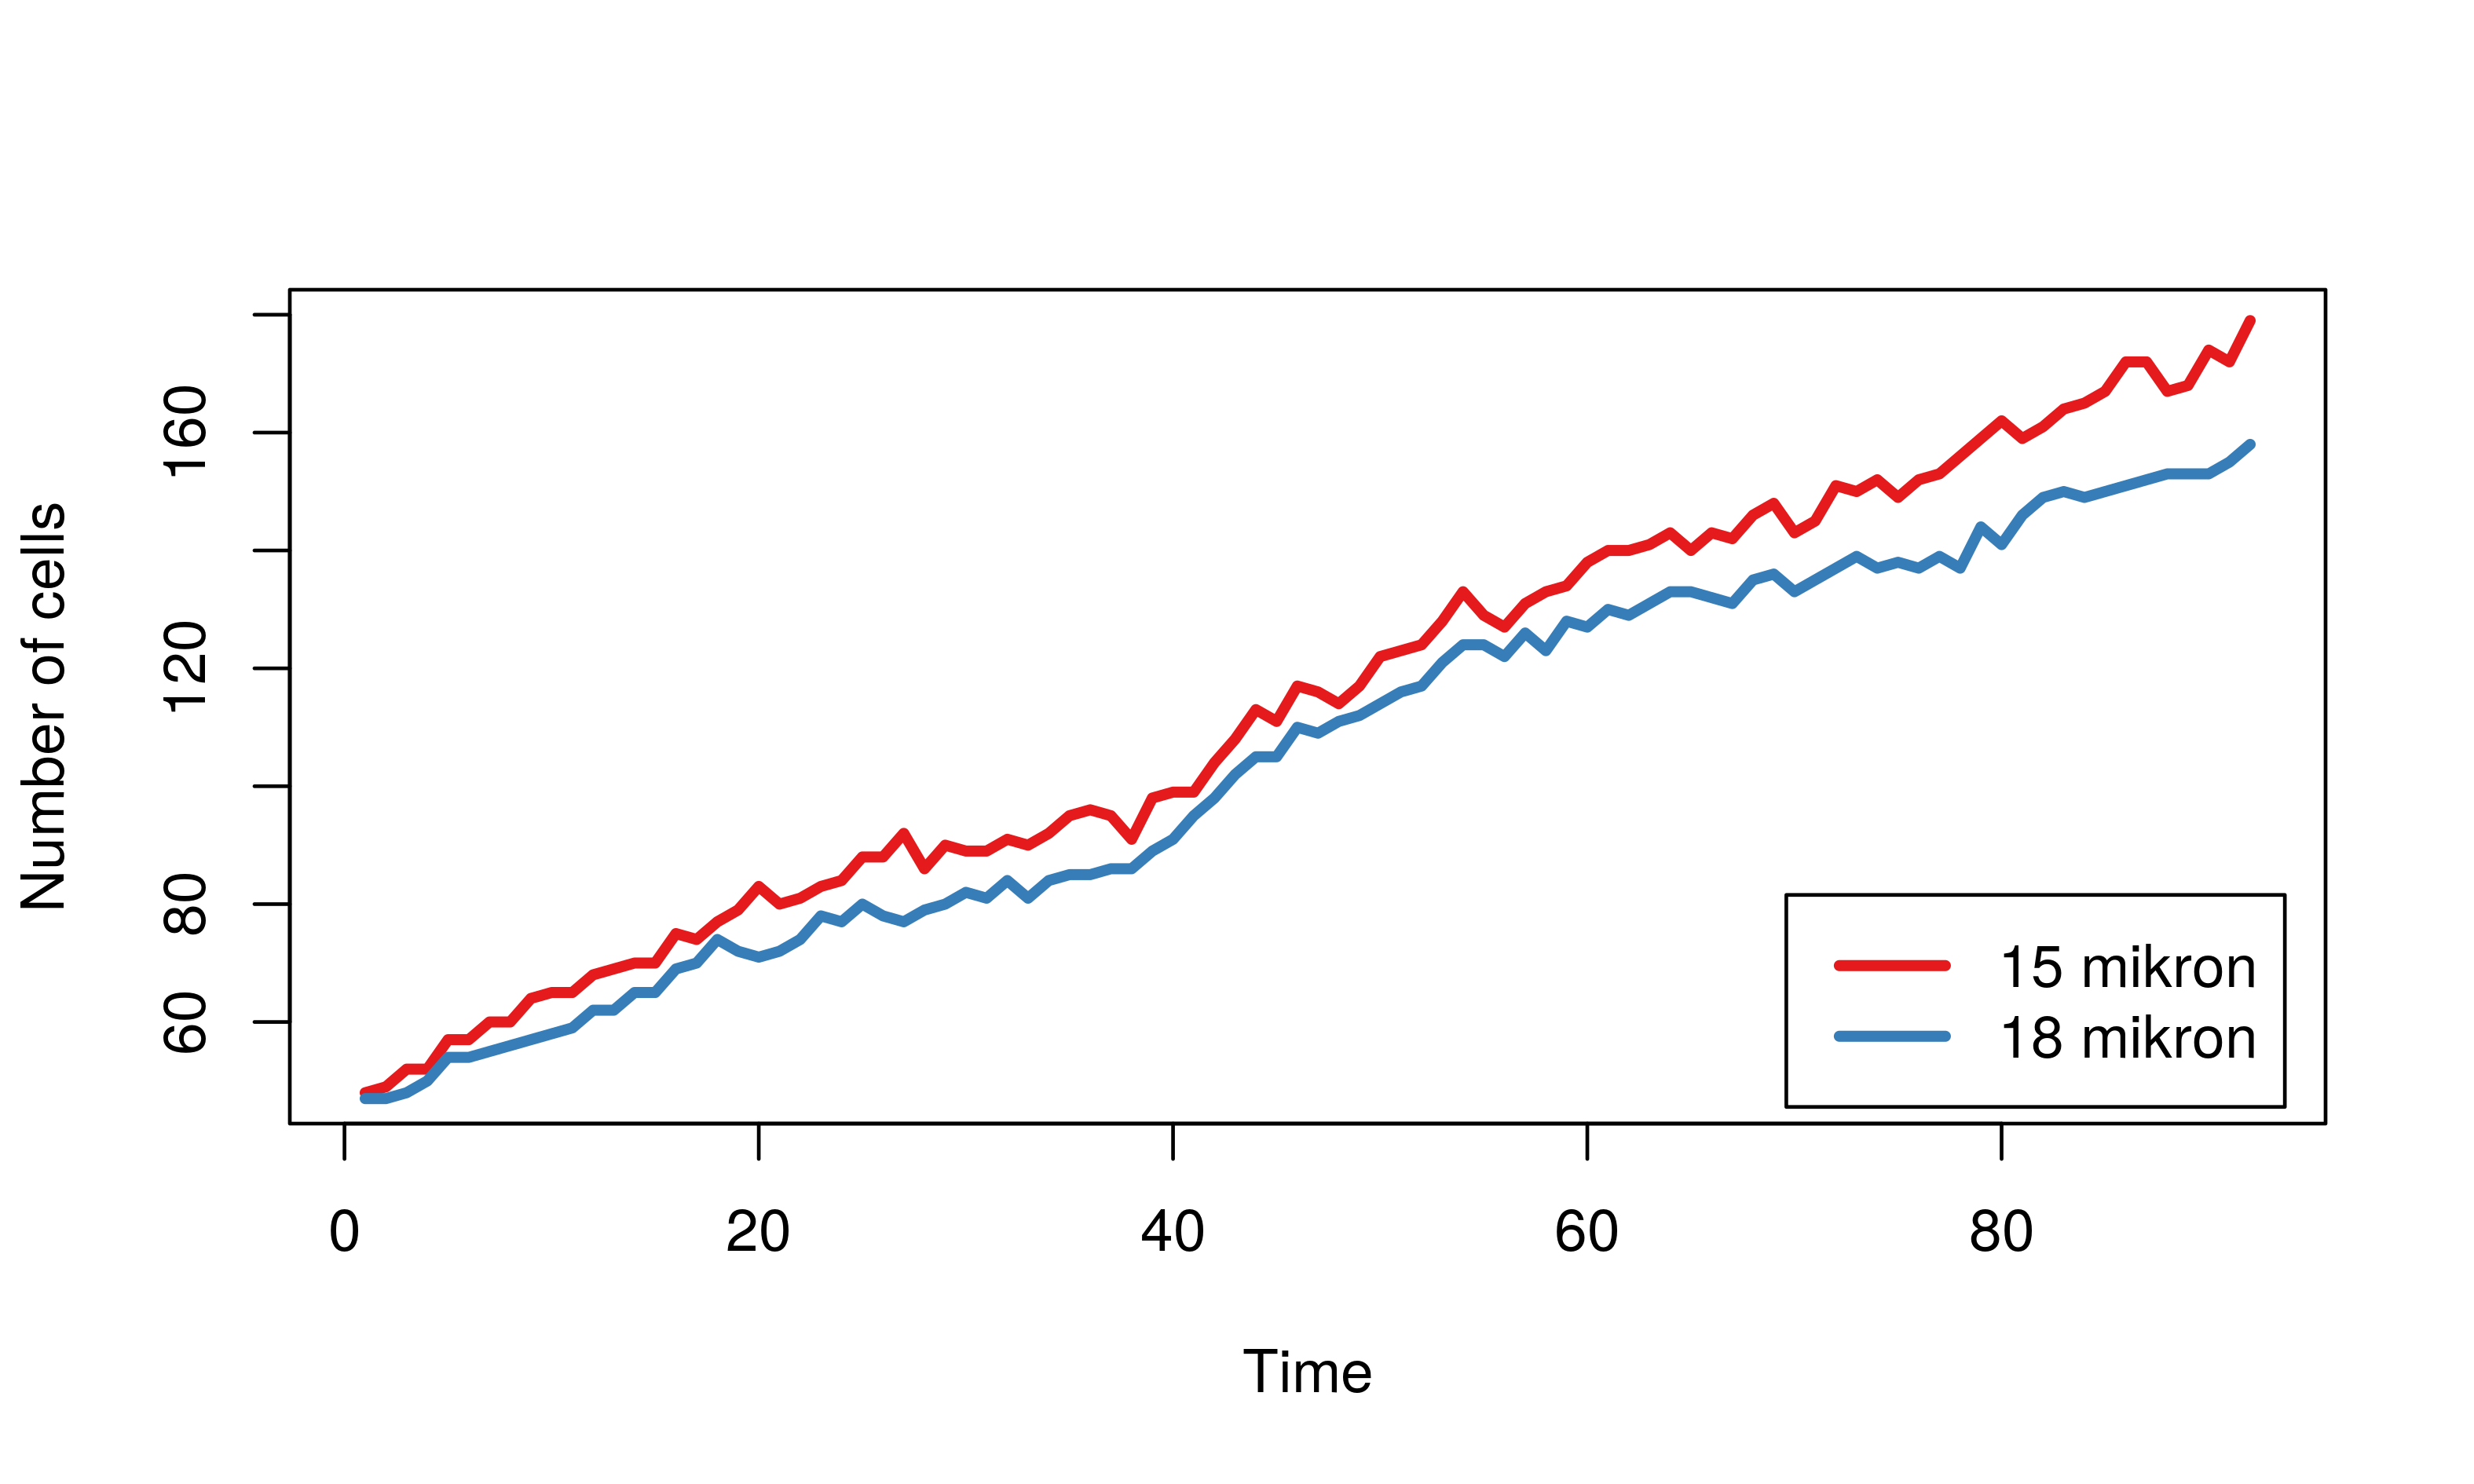
\includegraphics[width=\maxwidth]{figure/twocolumn-2_cells_per_time-1} 

}

\caption[Number of cells identified in total, as time progresses]{Number of cells identified in total, as time progresses. We note a linear in our time span, but note that we in a longer time-series would likely observe exponential growth. The two lines signify simulations using TrackMate with different estimated blob sizes. With a smaller estimate, the sensitivity is higher, and more cells are able to be identifies. However, this comes at the cost of losing more tracks when filtering, due to more cells dropping in and out during the time course.}\label{fig:2_cells_per_time}
\end{figure}
\end{Schunk}



% Doing our analysis, we note that only length(all.splits.init) of our initial 48 tracks are recovered after pruning away the ones which contain cells that disappear. These tracks collectively have a mean number of cell division events of $round(mean.cell.div, 2) \pm round(stds.cell.div, 2)$. If we instead choose not to filter on presence at the beginning, the number of division events reach $round(mean.cell.div.tot, 2) \pm round(stds.cell.div.tot, 2)$. 

Investigating the number of cell division events can be seen in \cref{tab:tracks}, where denoted filtering methods have been applied in the calculations. As we can see, when not filtering at all, and utilize all 48 tracks, the mean is still within the range of the pruned answers. In particular, when filtering out cells that fall within 20 pixels of the boundaries (ca $31~\mu m$), we achieve a result very similar to the ones where we filter away all the tracks where any cell at any point disappear.

\begin{table*}
  \centering
  \caption{Table description of the different simulations and their corresponding input parameters and results.}
  \label{tab:tracks}
  \begin{tabular}{cccc}\toprule
  \emph{Filter} & \emph{Number of tracks} & \emph{Mean} & \emph{SE} \\\midrule
    None          & 48 & 2.02 & 0.25 \\
    Edges         & 35 & 2.31 & 0.28 \\
    Disappearance & 17 & 2.71 & 0.44 \\\bottomrule
  \hline
  \end{tabular}
\end{table*}

\begin{figure}[H]
  \centering
  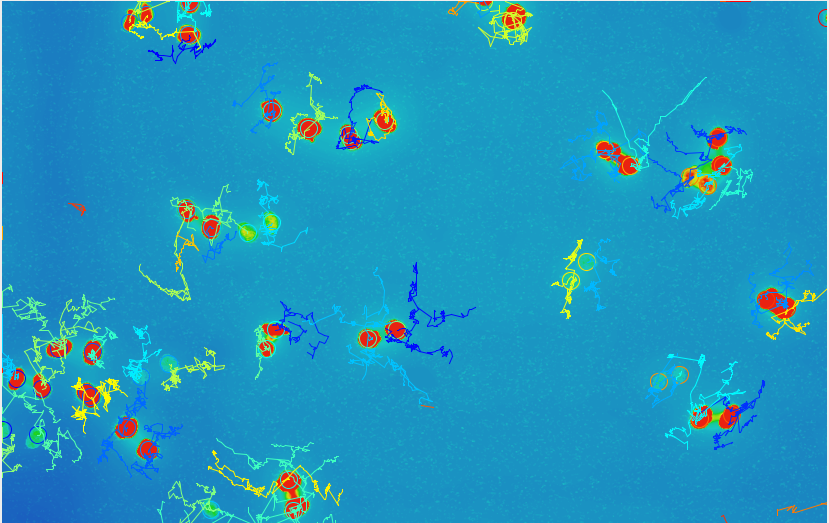
\includegraphics[width=.5\textwidth]{../figures/start_cells.png}
  \caption{Cells and subsequenct tracks at the first frame, using an estimated blob size of 15 $\mu m$.}
  \label{fig:contrasts}
\end{figure}
\begin{figure}[H]
  \centering
  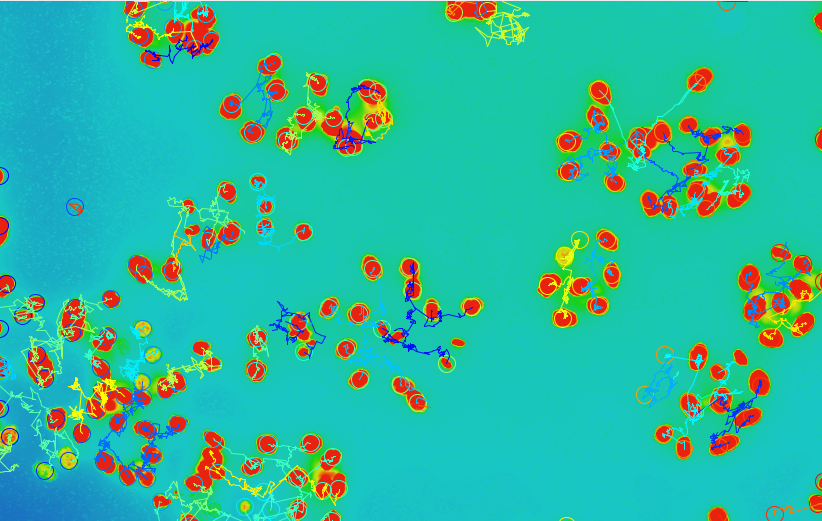
\includegraphics[width=.5\textwidth]{../figures/end_cells.png}
  \caption{Cells and tracks at the last frame. Occasional new tracks appear, as can be seen on the lonely, scattered lines appearing at a distance from the other clusters. }
  \label{fig:contrasts}
\end{figure}

Naturally, our method suffers from several drawbacks that are all hard to circumvent. The perhaps msot obvious one is the requirement of cells to be within view throughout the simulation, which is what causes the most drastic loss in tracks when filtering. In several cases, cells simply fall outside the x-y boundaries, where exclusion is more reasonable. However, when a cell drops out of view in the z-dimension, it is not as clear whether we should exclude it or not, since there is often some sort of visual cue that the cell is still present, even though the segmentation is not able to identify it. A similar problem occurs when cells come too close to each other in such a way that their intensities overlap such that they become indistinguishable from each other, and we are again forced to exclude the whole track from the analysis. In addition, the same thing happens during mitosis, when the chromosomes align and become thin, as we are attempting to identify the targets as approximately spherical (circular).

There is also a problem with identifying what cells belong to a certain track due to cell division events that cause one of the offspring to occur in a far-away position. The risk is that this new cell, which is supposed to be considered a part of the same track as the other cell, is simply regarded as a completely new track on its own. Having a higher allowed split distance would work as a counter to this, but would instead suffer from misidentifying cells coming in from outside the field of vision as cell division events, which we definitely do not want. Similarly, allowing for a higher number of frames for where a cell can be absent while still considering it to be part of the track when it reappears introduces the problem with replacing a cell with another one which just so happens to be in a position where the factual cell could have been.

However, despite the many problems with this general approach, we see merit in many parts of applying it as a type of preprocessing. In several cases, TrackMate is able to identify candidate cells which would be harder to manually justify. We also get the benefit of consistency -- whereas a human doing manual tracking would primarily evaluate cells based on their visual appearance, TrackMate only considers the hard numbers, which makes its classification well-defined and concise. There is naturally also the benefit of using the automated approach as primarily complementary, and simply pruning the results from our algorithms manually afterwards. Still, while using software to do the main body of the tracking is indeed automated, there are high amounts of manual tweaking which has to be done beforehand, in addition to the post-tracking adjustments. Many of these settings are fairly arbitrary, and it is hard from the viewpoint of the user to be able to determine what makes the algorithm perform optimally. Often the preprocessing is done based on what is perceived as the most visually compelling, which is not necessarily what is optimal for the algorithm. In other words, while there are many helpful results coming out of the tracking as done here, there are many unresolved questions of how to improve on the results significantly. Still, the analysis itself can often be adapted to allow for insightful results; investigating the number of cell division events only requires us to be able to identify when a cell is undergoing mitosis, and only makes up a small fraction of all the events taking place in the time-series, which in addition also makes them significantly easier to manually correct in retrospect.

Track files can be downloaded at \url{https://www.dropbox.com/s/2xpof5hhz6yid0n/N2DL-HeLa_Tracks.xml?dl=0} (15~$\mu m$) and \url{https://www.dropbox.com/s/evx95zriehyb5fr/N2_Tracks.xml?dl=0} (18~$\mu m$).

\bibliography{references}
\end{multicols*}
\newpage
\appendix
\section{Code}
  \lstinputlisting{../code/process_embryo.ijm}
  \lstinputlisting{../code/plot_maxima.R}
  \lstinputlisting{../code/plot_tifs.R}
  \lstinputlisting{../code/estimate_and_plot_area.R}
  \lstinputlisting{../code/preprocess_tracking.ijm}
  \lstinputlisting{../code/analyse_tracks.R}
\end{document}
